\section{Algorytm Simulated Annealing}

%%%%%%%%%%%%%%%%
\begin{frame}{Typowa funkcja celu}
		Niezbędne:
		\begin{itemize}
			\item $C_i$ - reprezentacja konfiguracji układu
			\item $g(C_i)$ - funkcja celu
			\item procedura generacji kolejnych konfiguracji
		\end{itemize}
	\end{frame}	
	\begin{frame}{Algorytm Simulated Annealing}
		\begin{figure}
			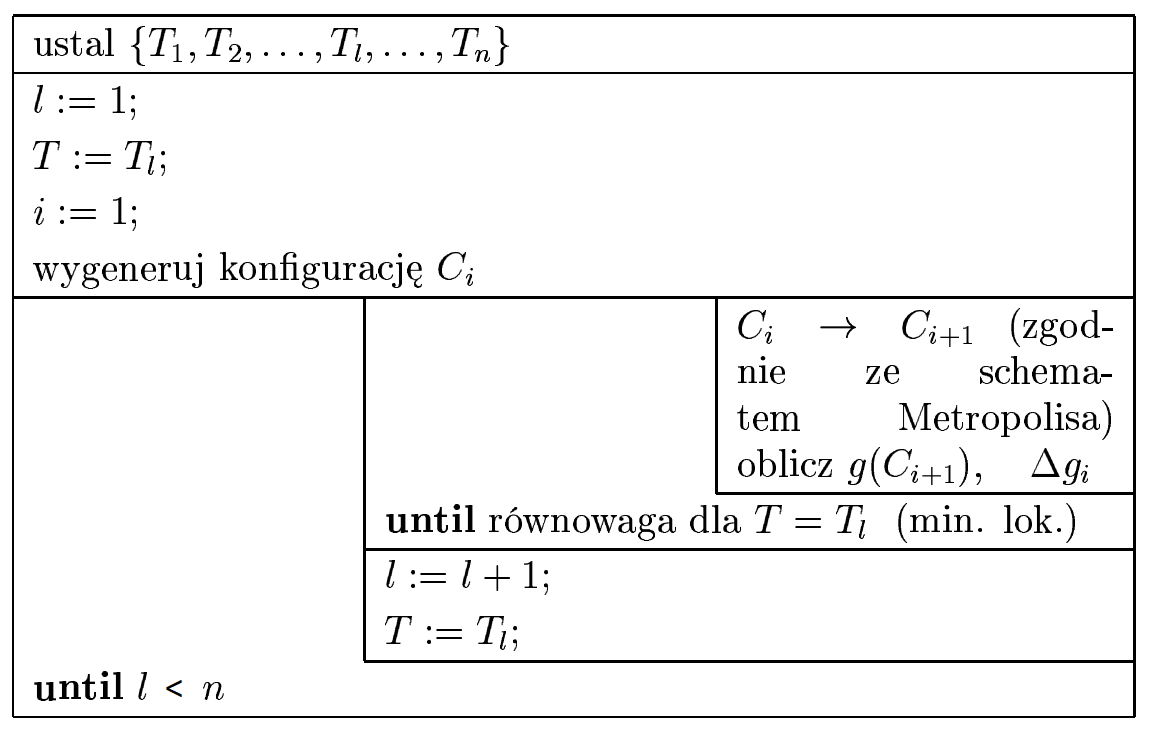
\includegraphics[width=0.8\textwidth]{img/18/sa_algorithm}
		\end{figure}
		$\{T_l\}$ - temperature schedule: $T_l > T_{l+1}$\\
		np. $T_{l+1} = 0.9 \cdot T_l$
	\end{frame}

	\begin{frame}{Fundamentalny fakt z mechaniki statystycznej}
		Załóżmy, że układ znajduje się w równowadze termicznej (w temperaturze $T$)\\
	Prawdopodobieństwo, że układ znajduje się w mikrostanie  stanie $\alpha$ jest proporcjonalne do {\bf czynnika Boltzmanna}  $$e^{\frac{-E_\alpha}{k_B T}}$$\\
		gdzie: $E_\alpha$ - energia stanu
	
		
		
	\end{frame}

%%%%%%%%%%%%%%%%

	\begin{frame}{Schemat Metropolisa}
		\textbf{Podstawa metody Monte Carlo symulacji molekularnej}
		\begin{figure}
			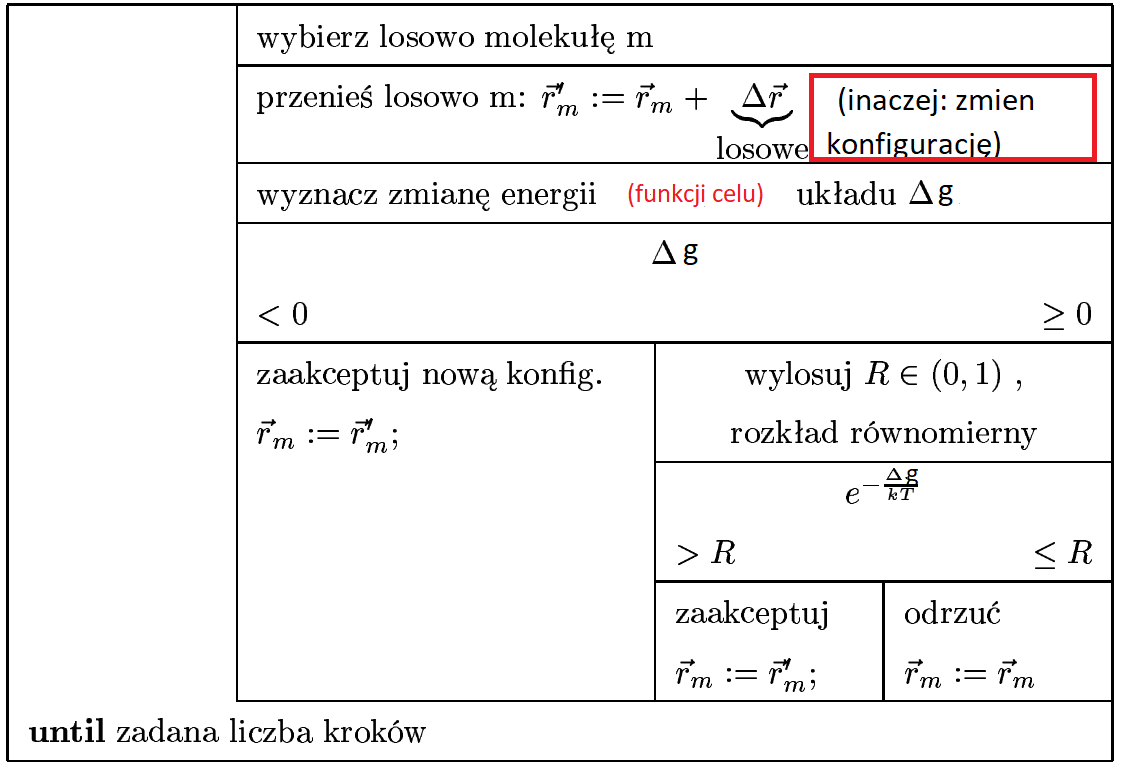
\includegraphics[width=0.67\textwidth]{img/18/metropolis1}
		\end{figure}
		\begin{thebibliography}{9}
			\setbeamertemplate{bibliography item}[article]
			\bibitem{metropolis}{Nicolas Metropolis, Arianna W. Rosenbluth, Marshal M. Rosenbluth, Augusta H. Teller, Edward Teller \newblock J. Chem. Phys. 21 (1953) 1087}
		\end{thebibliography}
	\end{frame}
		\begin{frame}{Sprawdzanie, czy układ jest w równowadze}
		\begin{block}{Sposób A}
			utrzymywać $T_l$ przez $\begin{cases}
			100 \cdot N \text{ prób} \\
			10 \cdot N \text{ prób udanych} (\Delta g < 0)
			\end{cases}$
		\end{block}
		
		\begin{block}{Sposób B}
		$n$ - ustalona liczba prób ($\sim$ epoka)
		\begin{enumerate}
			\item wykonać $n$ prób ($C_i \rightarrow C_{i+1}$)
			\item zachować g(C$_n$)
			\item porównać $g_i(C_n)$ dla kilku ostatnich zestawów po $n$ próbach \\
			brak istotnej zmiany $g(C_n) \rightarrow$ nowe $T$.
		\end{enumerate}
		\end{block}
\end{frame}
\begin{frame}{Wartość początkowa T}
\begin{itemize}
    \item wystarczająco wysoka by zapewnić akceptację niemal wszyskich przejść
    \item wartość początkowa parametru T zależy od postawionego problemu
    \item np. przyjąć jakiś wstępną wartość prawdopodobieństwa $P\approx 1$  i dla losowej próby wyliczyć średnią różnicę pomiędzy
    $\Delta g=g(C_i)-g(C_j)$
    \item wybrać $T_0=-\frac{\Delta g}{ln(P)}$
\end{itemize}
		   
			
		
		
\end{frame}
		\begin{frame}{Charakterystyka schematu Metropolisa}
		\begin{itemize}
			\item $T \nearrow$ - łatwiej akceptowalne kroki z $g(C_i) \nearrow (E)$ \\ $ \Rightarrow$ możliwość opuszczenia stanu metastabilnego (lokalnego minimum).
			\item zmiany $g(C_i) \searrow$ są akceptowane zawsze
		\end{itemize}
		
		Po wielu krokach system $\rightarrow$ stan równowagi termodynamicznej z parametrami oscylującymi wokół wartości średnich zgodnie z rozkładem Boltzmanna 
		

	\end{frame}

%%%%%%%%%%%%%%%%
%	\begin{frame}{Interaktywna demonstracja działania Simulated Annealing}
%		Źródła w C i C++:
%		\begin{itemize}
	%		\item 	%\url{https://www.taygeta.com/annealing/simanneal.html}
%		\end{itemize}
		
		
		%Programy w C:
		%Postscript:
		% martwe linki
%	\end{frame}